\section{Ricerca interna}\label{ricerca}

In piattaforme come TicketOne, dove l'utente è messo davanti ad una miriade di categorie ed ha a disposizione un'ampia scelta di eventi collocati in tutta Italia (e non solo), la ricerca diventa una parte essenziale.
\par Nel sito qui in analisi questa viene enfatizzata sin dall'homepage, visibile in Fig.~\ref{homepage}.
Una prima barra di ricerca è presentata all'interno dell'header mentre sulla parte sinistra della pagina sono presenti le principali categorie di eventi e le principali località italiane, in maniera che l'utente, anche se non sa esattamente cosa sta ricercando, possa capire cosa offre il sito e il territorio su cui opera.

\subsection{Barra di ricerca}

	Come accennato precedentemente, la barra di ricerca è posizionata all'interno dell'header ed è presente su quasi ogni pagina dinamica.
	\par Una semplice ricerca della parola ``\textit{teatro}'' (Fig.~\ref{ricerca1}) mostra come vi sia una funzione che popola la lista dei risultati parziali all'inserimento di ciascun carattere da parte dell'utente.
	I risultati presentati all'utente sono appunto parziali e mostrano le categorie in cui è presente la parola cercata.
	Nel caso specifico della Fig.~\ref{ricerca1}, si può vedere che la parola ``\textit{teatro}'' è presente in più categorie, come ad esempio: \textit{Artisti}, \textit{Luoghi evento}, \textit{Eventi}, ecc..
	\'E inoltre possibile cliccare su uno dei risultati presentati al momento della ricerca per poter andare direttamente nella pagina relativa a questo.
	
	\begin{figure}[hbt]
		\centering
		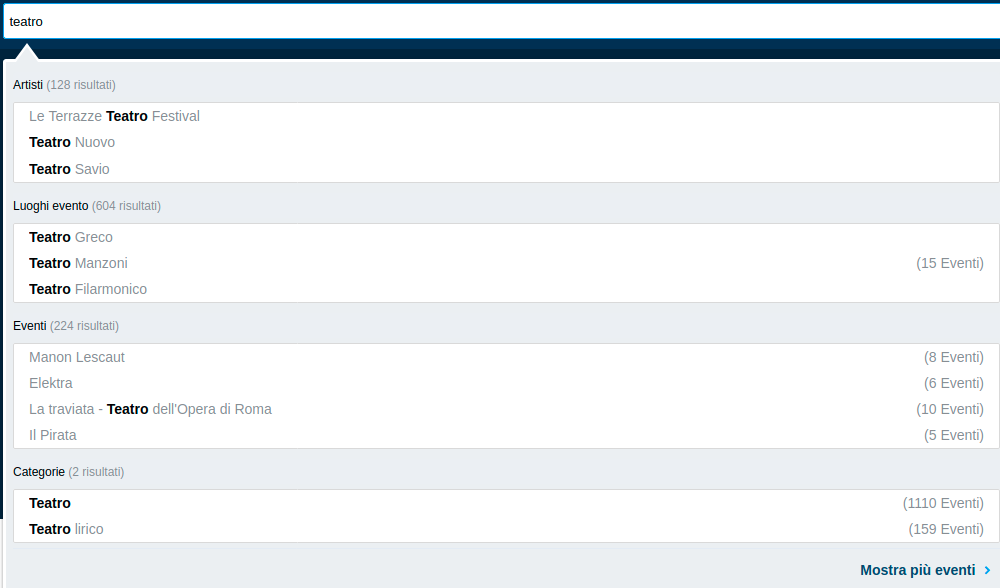
\includegraphics[width=\textwidth]{img/ricerca_1.png}
		\caption{Ricerca della parola teatro e suggerimenti}
		\label{ricerca1}
	\end{figure}

	I risultati vengono presentati in lista in base al match con il testo (Fig.~\ref{ricerca2}).
	Sulla colonna di sinistra è possibile vedere la categoria in cui si trovano i risultati ed è possibile scegliere di visualizzarne uno in particolare.
	
	\begin{figure}[hbt]
		\centering
		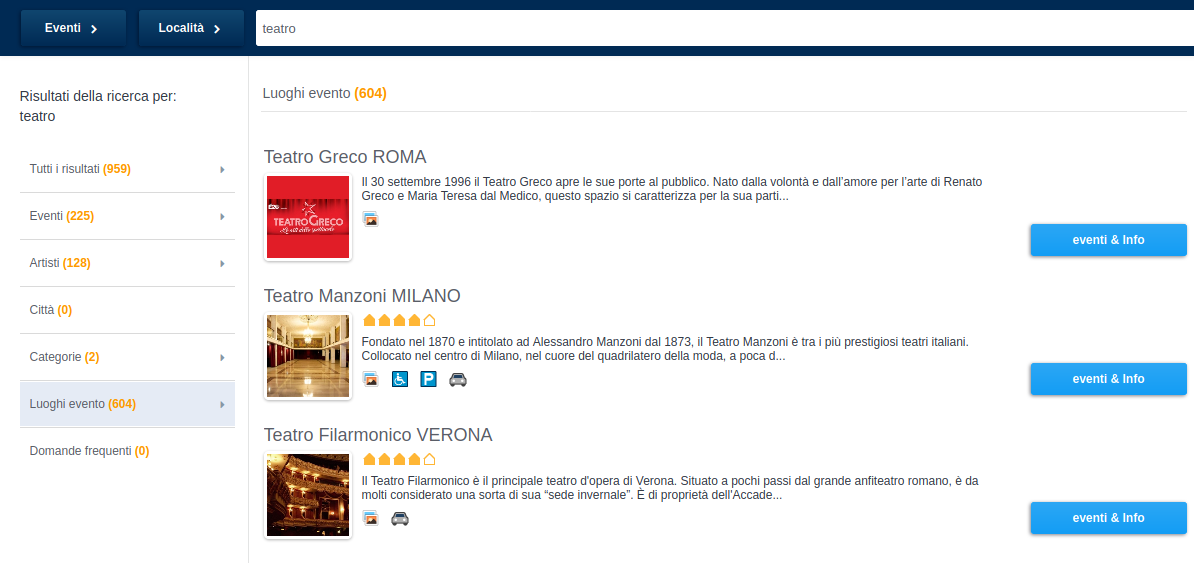
\includegraphics[width=\textwidth]{img/ricerca_2.png}
		\caption{Presentazione dei risultati relativi alla parola ``\textit{testo}''}
		\label{ricerca2}
	\end{figure}

\subsection{Ricerca avanzata}

	La ricerca ``semplice'' fornita dal sito è già molto completa in quanto permette di potersi muovere tra le categorie; tuttavia TicketOne fornisce anche una metodologia di \textit{ricerca avanzata} che permette all'utente di cercare più approfonditamente inserendo una maggior quantità di parametri (Fig.~\ref{ricerca3}).
	
	\begin{figure}[hbt]
		\centering
		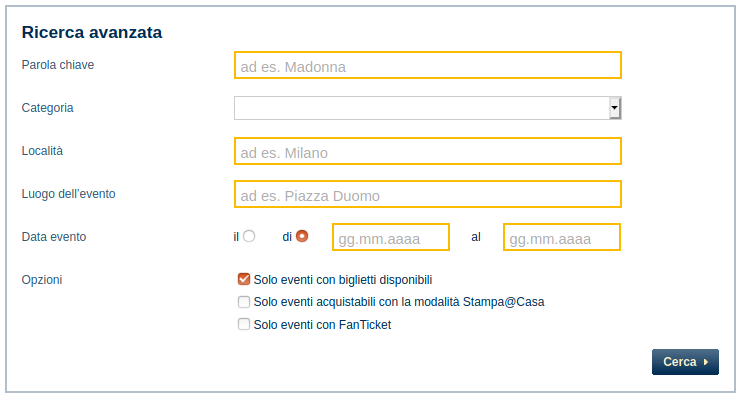
\includegraphics[width=\textwidth-.95cm]{img/ricerca_3.png}
		\caption{Box di ricerca avanzata}
		\label{ricerca3}
	\end{figure}

	Questa ricerca è \textit{statica} in quanto i risultati vengono mostrati solamente quando l'utente clicca il pulsante cerca.
	\'E in quel momento che questo viene reindirizzato ad una pagina con la lista dei risultati che possono essere ordinati in base alla tipologia di eventi, alla loro località e alla data in cui si svolgono.
	Tali parametri possono variare in base alla ricerca che è stata fatta.
	
	\begin{figure}[hbt]
		\centering
		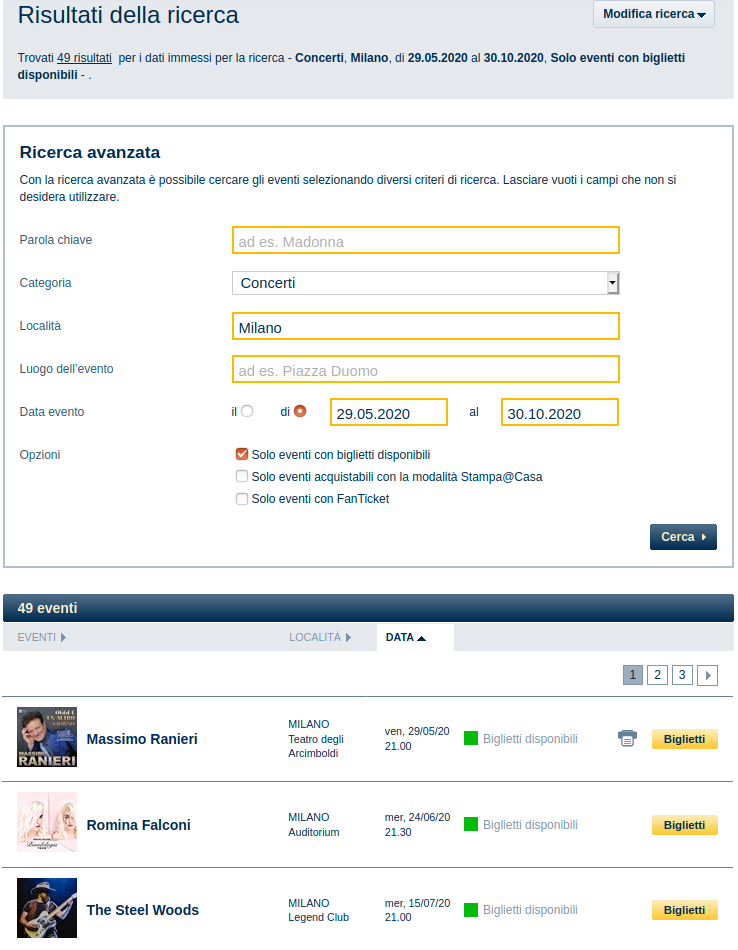
\includegraphics[width=\textwidth-.75cm]{img/ricerca_4.png}
		\caption{Risultati di una ricerca avanzata}
		\label{ricerca4}
	\end{figure}

\subsection{Considerazioni sulla metodologia di ricerca interna}

	\par La soluzione scelta da TicketOne per la ricerca è \textit{ibrida}, cioè i risultati vengono presentati all'utente mentre questo ancora sta scrivendo la parola da cercare, ma solamente in maniera parziale: questi sono i \textit{suggerimenti di ricerca}.
	Quando l'utente premerà il pulsante ``\textit{Cerca}'' a fianco della barra, allora verrà rimandato nella pagina con la lista di tutti i risultati.
	\par Questa scelta potrebbe risultare negativa in caso l'aggiornamento costante dei risultati distragga troppo l'utente o abbia tempi di caricamento eccessivi che portino a considerare l'uso del sito un'esperienza negativa.
	In questo caso specifico, tuttavia, non vi è alcun appesantimento del sito in quanto è presente solamente una lista parziale dei risultati per permettere all'utente di poter navigare più velocemente in caso trovasse direttamente la pagina di suo interesse.
	\par In generale lo strumento di ricerca interna di TicketOne è altamente funzionale e \textit{user-friendly} in quanto permette all'utente di spostarsi facilmente tra le categorie di eventi e di ordinare i risultati trovati.
